\documentclass[tikz,border=8pt]{standalone}
\usepackage{amsmath}
\usetikzlibrary{arrows.meta,calc,fit,backgrounds}

\definecolor{forwardblue}{RGB}{50,92,140}
\definecolor{backorange}{RGB}{204,93,39}
\definecolor{nodefill}{RGB}{247,250,252}
\definecolor{splitfill}{RGB}{232,245,243}
\definecolor{sumfill}{RGB}{255,249,230}
\definecolor{outfill}{RGB}{238,219,238}
\definecolor{notefill}{RGB}{245,247,250}
\definecolor{ink}{RGB}{23,32,51}

\begin{document}
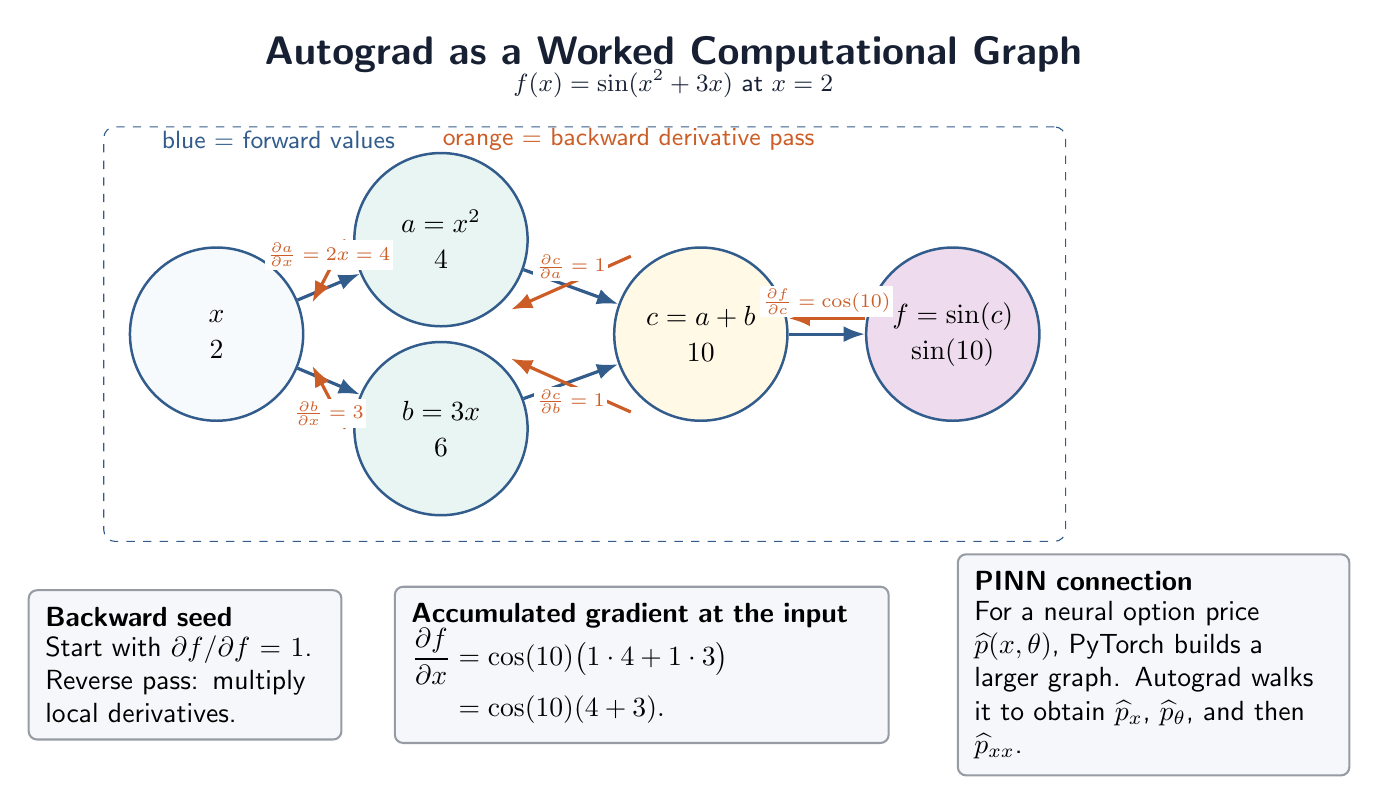
\begin{tikzpicture}[
    font=\sffamily,
    value/.style={
        circle,
        draw=forwardblue,
        fill=nodefill,
        line width=0.9pt,
        minimum size=22mm,
        align=center,
        inner sep=2pt
    },
    fwd/.style={-{Latex[length=2.7mm]}, forwardblue, line width=1.15pt},
    back/.style={-{Latex[length=2.7mm]}, backorange, line width=1.15pt},
    local/.style={font=\scriptsize, text=backorange, fill=white, inner sep=1pt},
    fwdlabel/.style={font=\scriptsize, text=forwardblue, fill=white, inner sep=1pt},
    note/.style={
        rounded corners=3pt,
        draw=ink!45,
        fill=notefill,
        line width=0.75pt,
        align=left,
        inner sep=6pt
    }
]

\node[align=center, font=\sffamily\bfseries\Large, text=ink] at (0.2,3.55)
    {Autograd as a Worked Computational Graph};
\node[align=center, font=\sffamily\small, text=ink] at (0.2,3.18)
    {$f(x)=\sin(x^2+3x)$ at $x=2$};

% Forward value graph.
\node[value] (x) at (-5.6,0.0) {$x$\\[1pt]$2$};
\node[value, fill=splitfill] (a) at (-2.75,1.2) {$a=x^2$\\[1pt]$4$};
\node[value, fill=splitfill] (b) at (-2.75,-1.2) {$b=3x$\\[1pt]$6$};
\node[value, fill=sumfill] (c) at (0.55,0.0) {$c=a+b$\\[1pt]$10$};
\node[value, fill=outfill] (f) at (3.75,0.0) {$f=\sin(c)$\\[1pt]$\sin(10)$};

\draw[fwd] (x) -- (a);
\draw[fwd] (x) -- (b);
\draw[fwd] (a) -- (c);
\draw[fwd] (b) -- (c);
\draw[fwd] (c) -- (f);

% Reverse derivative pass on the same graph.
\draw[back] ([yshift=2.0mm]f.west) -- node[local, above] {$\frac{\partial f}{\partial c}=\cos(10)$} ([yshift=2.0mm]c.east);
\draw[back] ([xshift=-1mm,yshift=2mm]c.north west) -- node[local, above] {$\frac{\partial c}{\partial a}=1$} ([xshift=1mm,yshift=-1mm]a.south east);
\draw[back] ([xshift=-1mm,yshift=-2mm]c.south west) -- node[local, below] {$\frac{\partial c}{\partial b}=1$} ([xshift=1mm,yshift=1mm]b.north east);
\draw[back] ([xshift=-1mm]a.west) -- node[local, above] {$\frac{\partial a}{\partial x}=2x=4$} ([xshift=1mm,yshift=4mm]x.east);
\draw[back] ([xshift=-1mm]b.west) -- node[local, below] {$\frac{\partial b}{\partial x}=3$} ([xshift=1mm,yshift=-4mm]x.east);

% Explanatory panels are separated from the graph to keep the illustration uncluttered.
\node[note, text width=3.55cm] (seed) at (-6.0,-4.2)
    {\textbf{Backward seed}\\[-1pt]
    Start with $\partial f/\partial f=1$. Reverse pass: multiply local derivatives.};

\node[note, text width=5.85cm] (chain) at (-0.2,-4.2)
    {\textbf{Accumulated gradient at the input}\\[-1pt]
    $\displaystyle
    \begin{aligned}
    \frac{\partial f}{\partial x}
    &=\cos(10)\bigl(1\cdot 4+1\cdot 3\bigr)\\[-1pt]
    &=\cos(10)(4+3).
    \end{aligned}$};

\node[note, text width=4.55cm] (pinn) at (6.3,-4.2)
    {\textbf{PINN connection}\\[-1pt]
    For a neural option price $\widehat p(x,\theta)$, PyTorch builds a larger graph. Autograd walks it to obtain $\widehat p_x$, $\widehat p_\theta$, and then $\widehat p_{xx}$.};

\node[draw=forwardblue, rounded corners=4pt, dashed, fit=(x)(a)(b)(c)(f), inner sep=9pt] {};
\node[font=\sffamily\small, text=forwardblue, anchor=west] at (-6.42,2.47)
    {blue = forward values};
\node[font=\sffamily\small, text=backorange, anchor=west] at (-2.85,2.47)
    {orange = backward derivative pass};

\end{tikzpicture}
\end{document}
